\documentclass[12pt]{standalone}
\usepackage{subcaption}
\usepackage{tikz}

\begin{document}
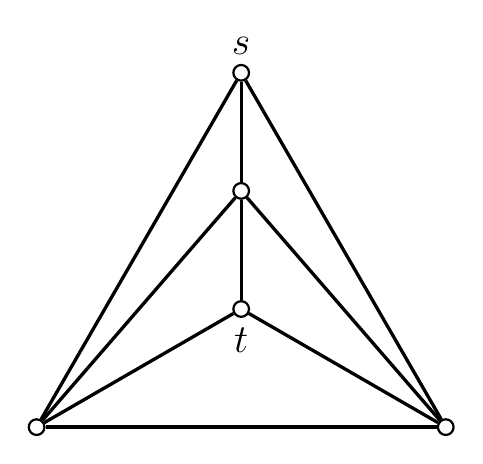
\begin{tikzpicture}[scale=1.5]
    \node[circle, thick, draw, inner sep=2pt, label={[text=black]below:{\Large $t$}}] (a) at (0:0) {};
    \node[circle, thick, draw, inner sep=2pt] (b) at (90:1) {};
    \node[circle, thick, draw, inner sep=2pt] (c) at (210:2) {};
    \node[circle, thick, draw, inner sep=2pt] (d) at (330:2) {};
    \node[circle, thick, draw, inner sep=2pt, label={[text=black]above:{\Large $s$}}] (e) at (90:2) {};
    \draw[very thick, black] (a) -- (b);
    \draw[very thick, black] (a) -- (c);
    \draw[very thick, black] (a) -- (d);
    \draw[very thick, black] (b) -- (c);
    \draw[very thick, black] (b) -- (d);
    \draw[very thick, black] (b) -- (e);
    \draw[very thick, black] (c) -- (d);
    \draw[very thick, black] (c) -- (e);
    \draw[very thick, black] (d) -- (e);
\end{tikzpicture}
\end{document}